\documentclass[runningheads]{llncs}
% PROVISIONAL: official Springer LLNCS class v2.26 (CTAN mirror of Springer's llncs package). Generated by build_main.py.
% (no T1 fontenc: avoids bitmap font generation)
\AtBeginDocument{\pdfpagewidth=210mm \pdfpageheight=297mm} % A4 PDF; llncs fixes only the 12.2x19.3 cm text block
\usepackage{graphicx}
\usepackage{booktabs}
\usepackage{amsmath,amssymb}
\usepackage{algorithm}
\usepackage{algpseudocode}
\usepackage{url}
\usepackage{array}
\setcounter{topnumber}{3}\setcounter{totalnumber}{5}\renewcommand{\topfraction}{0.9}\renewcommand{\bottomfraction}{0.8}\renewcommand{\textfraction}{0.1}\renewcommand{\floatpagefraction}{0.75}
\setlength{\textfloatsep}{8pt plus 2pt minus 2pt}\setlength{\floatsep}{8pt plus 2pt minus 2pt}\setlength{\intextsep}{8pt plus 2pt minus 2pt}\setlength{\abovecaptionskip}{4pt}
\begin{document}
\title{Does Dimensionality Reduction Help Classical Intrusion Detection? Original Features versus PCA and Kernel PCA on a Class-Stratified CIC-IDS2017 Sample}
\titlerunning{~}
\ifdefined\BLIND
\author{}
\authorrunning{~}
\institute{}
\else
\author{}
\authorrunning{~}
\institute{}
\fi
\maketitle
\begin{abstract}
Kernel principal component analysis (KPCA) is often paired with classical classifiers for network intrusion detection, yet its benefit over the original features needs a direct test. We compare the 78 original CIC-IDS2017 flow features with PCA and KPCA (linear, RBF and cosine kernels; 5 to 30 components) across five classifiers: logistic regression, $k$-nearest neighbours, SVM, decision tree and random forest. The data are a class-stratified sample of 6,000 records (at least 100 per class) drawn after exact duplicate removal; the sample does not preserve natural traffic prevalence. Imputation, scaling and reduction are fitted on training folds only. Evaluation combines repeated stratified cross-validation, nested cross-validation, a small nested hyper-parameter search, two row-order checks that serve as an unverified proxy for chronology , and a runtime and memory benchmark. A random forest on the original features scored highest; its best accuracy was 97.22\,\% (macro-F1 $0.901\pm0.020$; nested estimate $0.900\pm0.022$), yet two web-attack classes had F1 of only 0.53 and 0.59. Reduction did not help the decision tree or random forest and at best matched the original features for logistic regression and $k$-NN. Only the SVM gained from reduction (cosine KPCA), and that gain fell from 0.076 to 0.021 after tuning. In our benchmark, KPCA fitting took more than 200 times longer than PCA and whole-pipeline traced memory was about 37 times higher. The results come from one sample of one dataset, and every significance test carries a fold-dependence caveat.

\keywords{Network intrusion detection \and CIC-IDS2017 \and Kernel PCA \and Dimensionality reduction \and Class imbalance \and Machine learning.}
\end{abstract}

\section{Introduction}
Researchers usually build and compare network intrusion detection systems (NIDS) on public flow datasets, and CIC-IDS2017 is among the most common. Each flow in its MachineLearningCVE files has 78 numeric features. That invites dimensionality reduction, either to cut training cost or in the hope of generalizing better. Kernel PCA (KPCA) runs PCA in an implicit nonlinear feature space.

Such comparisons are hard to read for three reasons. First, CIC-IDS2017 is imbalanced, so the benign majority can dominate accuracy. Second, security datasets can leak information between training and test data, which inflates results. Third, saying that reduction helps means little without a no-reduction baseline, since otherwise the benefit is assumed, not measured. The IEEE Xplore studies surveyed in Section~\ref{sec:lit} illustrate these issues.

\textbf{Research questions.} \textbf{RQ1:} how does reduction change multi-class detection performance? \textbf{RQ2:} does KPCA beat the original space or ordinary PCA? \textbf{RQ3:} how do kernel, number of components and classifier interact? \textbf{RQ4:} what does reduction cost in time and memory? \textbf{RQ5:} do the conclusions hold under repeated class-aware validation, nested selection, tuning and row-order splits (a proxy for chronology)?

\textbf{Contributions.} (i) A reproducible comparison of the original features, PCA and three KPCA kernels over five classical classifiers, with fold-wise fitting, a majority-class baseline, a nested-CV check of selection optimism and a small nested hyper-parameter search, on a sample taken after exact same-label duplicate removal. (ii) A class-aware analysis of how far accuracy overstates detection quality. (iii) Paired statistical tests with an explicit independence caveat, plus two row-order robustness checks. (iv) A runtime and memory comparison of KPCA with PCA. We propose no new algorithm.

\section{Literature Survey}\label{sec:lit}
We reviewed 15 papers published in IEEE Xplore in 2025--2026 on intrusion detection with CIC-IDS2017 or closely related data. Table~\ref{tab:lit} gives the five with the highest accuracy stated for a multi-class or unspecified task; the other ten follow in the text. All values are quoted as the authors state them, mostly from the abstracts, and are not comparable across papers because datasets, splits and balancing differ.





\textit{Most accurate reported systems.} Pramana et al.~\cite{pramana} report an accuracy and F1 of 0.99996 for ridge-selected XGBoost and show that removing leakage features changes which features the SHAP analysis highlights. Qin~\cite{qin} reaches 0.9989 multi-class accuracy with a random forest on 20 selected features, but the macro-F1 is only 0.7114, so accuracy hides weak minority classes there as well. Patil and Joshi~\cite{patilj} propose an optimised attention-based deep network with 99.21\,\% accuracy. Ahuja and Vats Doohan~\cite{ahuja} compare four classical models, with XGBoost best at 97.73\,\% and the SVM weakest, and Amin and Jadhav~\cite{amin} balance classes with SMOTE before a random forest (97.6\,\%).

\textit{Dimensionality reduction.} Mosally~\cite{mosally} applies PCA to CICIDS2017, cutting 78 features to 33 while keeping 99\,\% of the variance, balances classes by SMOTE on the training data only, and finds a random forest better than an SVM; the abstract gives no figures. Zhang et al.~\cite{zhang} pair six classifiers with PCA, LDA and factor analysis and report that random forest with PCA performs best among the reduction pipelines; the abstract does not name the dataset. These two papers are the closest to our study, but their abstracts mention neither a class-level comparison against a no-reduction baseline nor KPCA.

\clearpage
\begin{table}[!t]
\caption{The five best papers of the survey (highest accuracy stated in the abstract for a multi-class or unspecified task) and this work. Values are quoted from each source and are not directly comparable.}\label{tab:lit}
\centering\scriptsize\setlength{\tabcolsep}{3pt}
\begin{tabular}{@{}p{0.55cm}p{3.1cm}p{3.7cm}p{1.9cm}p{2.2cm}@{}}
\toprule
Ref. & Paper details & Methodology & Dataset & Accuracy\\
\midrule
\cite{pramana} & Pramana, Putrada, Wicaksono; ICADEIS 2026 & Ridge feature selection with XGBoost; SHAP feature-stability analysis with leakage features removed & CICIDS2017 & 0.99996 (accuracy and F1)\\
\cite{qin} & Qin; ICNCIS 2025 & Random forest on top-20 flow features, SMOTE on training data, fuzzy rule layer & CIC-IDS2017 & 0.9989 multi-class (macro-F1 0.7114); 0.9995 binary\\
\cite{patilj} & Patil, Joshi; EITES 2025 & PMSpDN: modified split attention with a fused dyad network, weights tuned by Prairie Araneida optimisation & CIC-IDS2017 & 99.21\,\%\\
\cite{ahuja} & Ahuja, Vats Doohan; ICTBIG 2025 & XGBoost, random forest, LightGBM and SVM compared & ``CIC-IDS'' (version not stated) & 97.73\,\% (XGBoost)\\
\cite{amin} & Amin, Jadhav; ICONAT 2025 & SMOTE with random forest (200 trees) and engineered features & CICIDS2017 & 97.6\,\%\\
\midrule
\textbf{Ours} & This paper & Original features vs PCA vs linear/RBF/cosine KPCA; LR, $k$-NN, SVM, DT, RF & CIC-IDS2017, 6,000-record class-stratified sample & RF (original): 97.22\,\%; macro-F1 0.901\\
\bottomrule
\end{tabular}
\end{table}

\textit{Other recent classifiers on CIC-IDS2017.} Vankayalapati et al.~\cite{vank} use a random forest with recursive feature elimination and report 96.3\,\% multi-class and 99.9\,\% binary accuracy. G.P.\ et al.~\cite{gp} benchmark a random forest, XGBoost and a 1D-CNN, with the CNN at 96.34\,\% accuracy and a 3.01\,\% false-positive rate. Sharma and Kumar~\cite{sharma} use temporally separated splits and report an F1 of 99.6\,\% for XGBoost, 97.4\,\% for Isolation Forest and 94.7\,\% for HDBSCAN. Darmono et al.~\cite{darmono} study seven classes with synthetic augmentation and find boosting models near a macro-F1 of 0.973--0.976 whatever the augmentation, with bots as the main residual failure. Xu and Liu~\cite{xu} evaluate several models; in the arXiv version of their paper an MLP reaches 0.9775 accuracy on the overall test set but only 0.5863 on a test set of unknown attacks.

\textit{Dataset and evaluation issues.} Jiwueze and Varol~\cite{jiwueze} compare CIC-IDS-2017 with a revised dataset and conclude that tree models are more consistent than deep models on rare attacks and that dataset composition must be considered with model choice. Mohsin et al.~\cite{mohsin} find that random forest and decision tree perform better on engineered features than on raw ones. Bandarupalli~\cite{bandar} proposes a lightweight deep neural network for anomaly-based detection on CIC-IDS-2017; the abstract reports no figures.

These studies report high accuracy under different splits and balancing schemes, and only some report class-level metrics. We read only these 15 papers, mostly their abstracts, so we claim no gap in the literature.



\section{Proposed Work}\label{sec:proposed}
\textbf{Objectives.} The work answers the research questions above by a controlled comparison, not by a new algorithm: every feature space and classifier is evaluated under the same folds, with all data-dependent steps fitted on the training fold only. \textbf{Methodology in brief.} A class-stratified sample of 6{,}000 flows is drawn after duplicate removal; each classifier is trained on the original 78 features and on PCA or KPCA features; results are scored with accuracy, macro-F1 and MCC under repeated and nested cross-validation (Algorithm~\ref{alg:cv} and Fig.~\ref{fig:pipe}).

\subsection{Dataset and Preprocessing}\label{sec:data}
\textbf{Data.} We use the eight daily CIC-IDS2017 \texttt{MachineLearningCVE} files: 2{,}830{,}743 flows, 78 numeric features, 15 labels (counts computed from the files; no provider checksum was available). There is no timestamp column. Rows with missing or infinite values are 0.2\,\% or less of each file (inf $\to$ NaN) and were not imputed before sampling. Eight features are constant in every file and were kept to match the 78-feature definition of earlier work.

\textbf{Duplicates.} 308{,}381 flows (10.9\,\%) are exact duplicates (identical on all 78 features and the label) of another flow and were removed before sampling, because identical flows in training and test folds inflate scores. Feature-identical flows with \emph{different} labels were not removed: 698 such conflicting-label groups remain in the 2.52\,M pool. None of them fell into the 6{,}000-record sample: it contains no two records with identical feature vectors, with the same or with different labels. Duplication is uneven: removal took 43\,\% of PortScan flows (158{,}930 to 90{,}819) and 25\,\% of DoS Hulk flows, versus 7.8\,\% of benign flows.

\textbf{Sample.} Exact KPCA needs an $n\times n$ kernel matrix, so we draw a stratified random sample of 6{,}000 records from the de-duplicated pool of 2{,}522{,}362 flows (seed 0): each class contributes at least 100 records (all of them if fewer exist). The rest is allocated in proportion to pool prevalence. Heartbleed (11), SQL injection (21) and Infiltration (36) are therefore complete but tiny; the floor over-represents attacks (benign: 67.2\,\% of the sample versus 83\,\% of the pool). Sampling uses only labels and random numbers; \emph{no imputation or scaling statistic is computed before the split}. Only two feature cells in the sample are missing; they are imputed with training-fold means inside each fold. Each record keeps its source file (day) and row position for the row-order checks.



\subsection{Methodology}\label{sec:method}
\textbf{Pipeline.} Fig.~\ref{fig:pipe} shows the protocol. Within each training fold we fit a mean imputer and a standard scaler, then the dimensionality reducer; test folds are only transformed. Feature spaces are: \emph{original} (78 standardised features); \emph{PCA}; and \emph{KPCA} with linear, RBF (scikit-learn default $\gamma=1/78$) and cosine kernels , each with $n\in\{5,10,15,20,30\}$ components. The reducer is fitted once per fold and shared by all classifiers, which is equivalent to fitting it inside each pipeline because it is deterministic (unit-tested).


\textbf{Algorithm and formulas.} Algorithm~\ref{alg:cv} summarises one evaluation of a feature space and classifier. Features are standardised as $z_j=(x_j-\mu_j)/\sigma_j$ with $\mu_j,\sigma_j$ from the training fold. PCA projects onto the leading eigenvectors $\mathbf{v}_k$ of the training covariance matrix $\mathbf{C}=\frac{1}{n}\mathbf{Z}^{\top}\mathbf{Z}$. KPCA uses the kernel matrix $K_{ij}=k(\mathbf{z}_i,\mathbf{z}_j)$ with
\begin{equation}
k_{\mathrm{lin}}=\mathbf{z}^{\top}\mathbf{z}',\qquad k_{\mathrm{rbf}}=\exp(-\gamma\lVert\mathbf{z}-\mathbf{z}'\rVert^{2}),\ \gamma=\tfrac{1}{78},\qquad k_{\cos}=\frac{\mathbf{z}^{\top}\mathbf{z}'}{\lVert\mathbf{z}\rVert\,\lVert\mathbf{z}'\rVert},
\end{equation}
centred as $\tilde{K}=K-\mathbf{1}_nK-K\mathbf{1}_n+\mathbf{1}_nK\mathbf{1}_n$; with $\mathbf{1}_n$ the $n\times n$ matrix whose entries are all $1/n$. For the leading eigenpairs $(\lambda_k,\boldsymbol{\alpha}_k)$ of $\tilde{K}$, with $\lVert\boldsymbol{\alpha}_k\rVert=1$, a sample is projected to $\tilde{K}_{\mathrm{new}}\boldsymbol{\alpha}_k/\sqrt{\lambda_k}$, with $\tilde{K}_{\mathrm{new}}$ the centred kernel against the training fold (the same scaling as \texttt{KernelPCA.transform}). With per-class precision $P_c$ and recall $R_c$, the primary metric is
\begin{equation}
F1_c=\frac{2P_cR_c}{P_c+R_c},\qquad \text{macro-F1}=\frac{1}{C}\sum_{c=1}^{C}F1_c,\ \ C=15,
\end{equation}
and balanced accuracy equals macro-recall. The multi-class MCC from the confusion matrix $\mathbf{M}$ with $s$ samples, $t_k$ true and $p_k$ predicted counts of class $k$, and $c=\sum_k M_{kk}$ correct predictions is
\begin{equation}
\mathrm{MCC}=\frac{c\,s-\sum_k p_kt_k}{\sqrt{s^{2}-\sum_k p_k^{2}}\,\sqrt{s^{2}-\sum_k t_k^{2}}}.
\end{equation}



\begin{figure}[!htbp]\centering
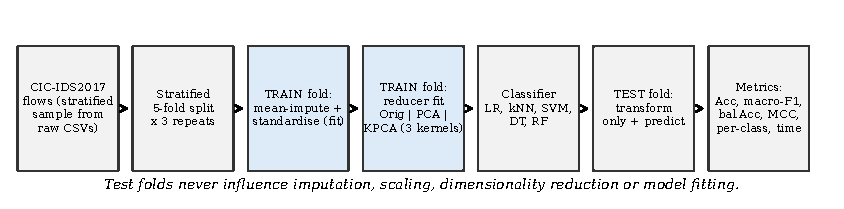
\includegraphics[width=0.62\textwidth]{figures/fig1_pipeline.pdf}
\caption{Experimental pipeline. All data-dependent preprocessing and reduction is fitted on the training fold only.}\label{fig:pipe}
\end{figure}



\textbf{Classifiers.} Logistic regression (L2, lbfgs), $k$-NN with $k=5$ , an SVM with RBF kernel, $C=1$ and $\gamma$=``scale'' , a decision tree with entropy criterion , and a random forest with 100 trees , using scikit-learn . The main grid uses these fixed default settings; a separate nested search (below) tests whether tuning changes the conclusions. Each classifier except $k$-NN is also run with \texttt{class\_weight=balanced}. A majority-class classifier is the trivial baseline. Resampling such as SMOTE is not used because Heartbleed has only 8--9 training records per fold.

\textbf{Validation.} Repeated stratified 5-fold cross-validation, 3 repeats (15 folds), seed 42; every method sees identical folds, giving paired observations. Test folds hold about 2 Heartbleed and 4 SQL-injection records, so those per-class estimates are noisy; we report means and standard deviations over 15 folds.

\begin{algorithm}[!t]
\caption{Fold-wise evaluation of one feature space $S$ and classifier $f$}\label{alg:cv}
\begin{algorithmic}[1]
\Require sample $(X,y)$ of 6,000 records; space $S\in\{$original, PCA, KPCA$(k,n)\}$; classifier $f$; 3 repeats of stratified 5-fold CV (seed 42)
\Ensure mean and standard deviation of accuracy, macro-F1, MCC and cost over 15 folds
\For{each repeat $r$ and fold $(\mathrm{tr},\mathrm{te})$}
 \State fit mean imputer and standard scaler on $X_{\mathrm{tr}}$; transform $X_{\mathrm{tr}}$ and $X_{\mathrm{te}}$
 \If{$S\neq$ original}
  \State fit reducer $T_S$ ($n$ components) on the scaled $X_{\mathrm{tr}}$ only
  \State $Z_{\mathrm{tr}}\gets T_S(X_{\mathrm{tr}})$;\ $Z_{\mathrm{te}}\gets T_S(X_{\mathrm{te}})$
 \Else
  \State $Z_{\mathrm{tr}}\gets X_{\mathrm{tr}}$;\ $Z_{\mathrm{te}}\gets X_{\mathrm{te}}$
 \EndIf
 \State fit $f$ on $(Z_{\mathrm{tr}},y_{\mathrm{tr}})$;\ predict $\hat{y}$ on $Z_{\mathrm{te}}$; record metrics and fit time
\EndFor
\State \Return mean $\pm$ std over the 15 folds (nested selection repeats this inside each outer training set with 3 inner folds)
\end{algorithmic}
\end{algorithm}

\textbf{Nested cross-validation for selection.} Picking the best of 189 configurations (21 feature spaces $\times$ 9 classifier and weighting variants) on the same folds that score it flatters the winner. To measure this, selection is nested: inside each of the 15 outer training sets (4{,}800 records) a stratified 3-fold inner cross-validation scores every configuration by macro-F1. The inner winner is then scored once, on the outer test fold it never saw. We run this for (A) the global choice and, for each classifier, for (C) the best \emph{reduced} space with weighting versus (D) the original space with weighting chosen the same way.

\textbf{Nested hyper-parameter search.} For $k$-NN, SVM and random forest on four spaces (original, PCA-30, KPCA-cosine-30, KPCA-RBF-30), a 3-fold inner cross-validation inside each of the first five outer folds selects from small grids: $k\in\{3,5,7,11\}$; SVM $C\in\{0.1,1,10\}$, $\gamma\in\{\text{scale},0.01,0.1\}$, class weight none/balanced; random forest 100/200 trees, depth none/10/20, class weight none/balanced. The RBF width of the KPCA reducer itself is not tuned.

\textbf{Row-order robustness checks (proxy chronology).} The raw files have no timestamps and attack flows occur in contiguous row blocks, so we \emph{assume}, without proof, that row order follows capture time. (i) \emph{Head/tail}: the first 70\,\% of each file's rows train, the last 30\,\% test. (ii) \emph{Blocked CV}: each file is cut into five contiguous blocks, each held out in turn. Only classes present in both training and test are scored, with a random split of the same rows and classes as comparator.

\textbf{Metrics.} Accuracy; macro-precision, macro-recall and macro-F1; weighted-F1; balanced accuracy; and the multi-class Matthews correlation coefficient (MCC) as implemented in scikit-learn. \textbf{Macro-F1 is the primary model-selection criterion}, chosen before the runs because it weights all 15 classes equally. Per-class results and the confusion matrix use pooled out-of-fold predictions of the first repeat.

\textbf{Statistics.} Per classifier we compare feature spaces at matched $n=10$ with two-sided Wilcoxon signed-rank tests on the 15 paired macro-F1 values, Holm-corrected over 30 comparisons (six per classifier: original vs PCA, RBF- and cosine-KPCA; PCA vs linear-, RBF- and cosine-KPCA; linear KPCA is not compared with the original because it reproduces PCA), with the rank-biserial correlation $r$ as effect size, and Friedman omnibus tests. Because folds share training data, the 15 differences are positively correlated and naive $p$-values are too liberal; we apply no correction for this and use the tests for screening, not as proof. Comparisons against each classifier's \emph{best} reduced space are selected on the same folds, which favours the reduced space; the nested analysis scores that selection on unseen outer folds.

\textbf{Cost.} A serial benchmark (no parallel workers) records training and inference time (median of 5 repetitions, one fold split) and peak memory from Python's \texttt{tracemalloc}, measured in a separate pass. Native allocations in compiled code are not traced, so memory figures are lower bounds.

\textbf{Setup.} A 2-vCPU, 7\,GB VM ran the main grid (2{,}850 fits = 190 configurations incl. the majority-class baseline $\times$ 15 folds; about 28 min), nested CV (about 64 min) and tuning (about 16 min).

\section{Results and Discussion}
\subsection{Original-feature baseline and the cost of reading accuracy alone}
A majority-class predictor already scores accuracy 0.672, with macro-F1 0.054 and MCC 0.000. The random forest on the original features reaches accuracy $0.972\pm0.004$ but macro-F1 $0.901\pm0.020$ (weighted-F1 0.971, balanced accuracy 0.883, MCC $0.948\pm0.008$). The 0.071 gap between accuracy and macro-F1 is driven by a handful of classes (Table~\ref{tab:perclass}). Ten of the 15 classes, among them benign, DDoS, the four DoS families, both Patator classes, PortScan and Heartbleed, have F1 $\ge$ 0.96. Web brute force (F1 0.53) and web XSS (0.59) are the weakest, and they are mostly confused with each other: 48 of 103 brute-force records are predicted as XSS, and 35 of 101 XSS records as brute force. Bot (0.87; recall 0.82), infiltration (0.875; recall 0.78 on 36 records) and SQL injection (0.84; 21 records) also fall short. We did not test whether labelling or feature-construction artefacts of the dataset explain this confusion.

\begin{table}[!htbp]
\caption{Per-class results of the selected model (RF, original features), pooled out-of-fold predictions, first repeat.}\label{tab:perclass}
\centering\scriptsize
\begin{tabular}{lrrrr}
\toprule
Class & Precision & Recall & F1 & Support \\
\midrule
BENIGN & 0.984 & 0.996 & 0.990 & 4034 \\
Bot & 0.924 & 0.817 & 0.867 & 104 \\
DDoS & 0.997 & 0.997 & 0.997 & 340 \\
DoS GoldenEye & 0.975 & 0.966 & 0.970 & 119 \\
DoS Hulk & 0.998 & 0.979 & 0.988 & 424 \\
DoS Slowhttptest & 0.955 & 0.973 & 0.964 & 110 \\
DoS slowloris & 1.000 & 0.927 & 0.962 & 110 \\
FTP-Patator & 1.000 & 1.000 & 1.000 & 111 \\
Heartbleed & 1.000 & 1.000 & 1.000 & 11 \\
Infiltration & 1.000 & 0.778 & 0.875 & 36 \\
PortScan & 0.989 & 0.981 & 0.985 & 270 \\
SSH-Patator & 1.000 & 0.943 & 0.971 & 106 \\
Web Brute Force & 0.581 & 0.485 & 0.529 & 103 \\
Web Sql Injection & 0.941 & 0.762 & 0.842 & 21 \\
Web XSS & 0.558 & 0.624 & 0.589 & 101 \\
\bottomrule
\end{tabular}

\end{table}





\subsection{Original space versus PCA versus Kernel PCA}
Table~\ref{tab:n10} and Fig.~\ref{fig:all} compare the feature spaces at $n=10$. Reduction usually hurt. The original space beat PCA-10 for logistic regression, SVM, decision tree and random forest, and beat RBF-10 and cosine-10 for all five classifiers; for $k$-NN it was indistinguishable from PCA-10 ($\Delta$ macro-F1 $-0.001$ from unrounded means 0.8005 and 0.8017). Of the 30 pairwise comparisons, 23 had Holm-adjusted $p<0.05$. Because folds share training data, we read these as screening evidence, not proof. Among the reduced spaces, RBF-KPCA was worse than PCA for LR, $k$-NN, DT and RF but better for the SVM. Cosine KPCA was better than PCA for the SVM ($+0.120$) and worse for LR, $k$-NN and DT. Linear KPCA never differed from PCA. The Friedman tests were all significant (Holm-adjusted $p\le 2.7\times10^{-9}$) and carry the same caveat.

A stricter question is whether each classifier's \emph{best} reduced space matches the original (table in the repository). These best spaces were picked on the same folds, which favours reduction. For DT ($+0.070$) and RF ($+0.056$) the original features were still better, in all 15 folds ($p_\mathrm{Holm}=0.0003$ for both). For logistic regression the best reduced space (PCA, 30 components) came within 0.004 (Holm-adjusted $p=0.021$ across the five best-space tests; because folds share training data, we treat this as exploratory, not definitive evidence of a difference). For $k$-NN there was no difference. The SVM is the one case where reduction helped: cosine KPCA with 30 components raised macro-F1 from 0.675 to 0.746 ($p_\mathrm{Holm}=0.0003$, better in all 15 folds). That gain needs many components; at 10 components cosine KPCA scores 0.605, below the original 0.675.

\begin{table}[!htbp]
\caption{Mean accuracy and macro-F1 at 10 components (original = 78 features); macro-F1 as mean $\pm$ std over 15 folds.}\label{tab:n10}
\centering\scriptsize
{\setlength{\tabcolsep}{7pt}\resizebox{\textwidth}{!}{\begin{tabular}{lccccc}
\toprule
Space & LR & KNN & SVM & DT & RF \\
\midrule
Original (78) & 0.924 / 0.736$\pm$0.022 & 0.934 / 0.800$\pm$0.024 & 0.906 / 0.675$\pm$0.017 & 0.964 / 0.881$\pm$0.021 & 0.972 / 0.901$\pm$0.020 \\
PCA-10 & 0.842 / 0.506$\pm$0.018 & 0.932 / 0.802$\pm$0.023 & 0.842 / 0.485$\pm$0.024 & 0.941 / 0.805$\pm$0.025 & 0.956 / 0.834$\pm$0.022 \\
KPCA-lin-10 & 0.842 / 0.507$\pm$0.017 & 0.932 / 0.802$\pm$0.023 & 0.842 / 0.485$\pm$0.024 & 0.942 / 0.806$\pm$0.024 & 0.957 / 0.836$\pm$0.019 \\
KPCA-RBF-10 & 0.805 / 0.306$\pm$0.015 & 0.918 / 0.757$\pm$0.029 & 0.880 / 0.525$\pm$0.016 & 0.920 / 0.755$\pm$0.037 & 0.937 / 0.790$\pm$0.037 \\
KPCA-cos-10 & 0.852 / 0.462$\pm$0.012 & 0.926 / 0.783$\pm$0.028 & 0.904 / 0.605$\pm$0.018 & 0.928 / 0.786$\pm$0.027 & 0.944 / 0.821$\pm$0.029 \\
\bottomrule
\end{tabular}
}}
\end{table}



Fig.~\ref{fig:all} shows all 25 classifier-by-space executions at 10 components (macro-F1, mean $\pm$ std over 15 folds; the black bar is the original space). Only for the SVM does a reduced space (cosine KPCA) beat the original, and the tree-based classifiers lead overall.

\begin{figure}[!t]\centering
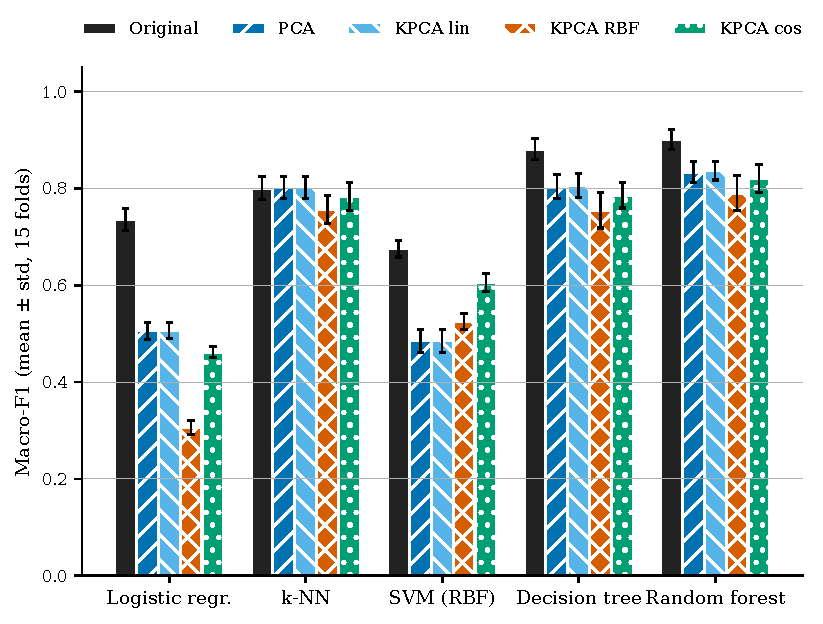
\includegraphics[width=0.95\textwidth]{figures/fig10_all_executions.pdf}
\caption{Macro-F1 of all classifier $\times$ feature-space executions at 10 components (mean $\pm$ std over 15 folds; standard class weights; axis starts at zero).}\label{fig:all}
\end{figure}

\subsection{Accuracy of each algorithm across feature spaces}
Fig.~\ref{fig:peralgo} shows one panel per classifier: bars give mean accuracy for PCA and the three KPCA kernels at 5 to 30 components, and the dashed line is the accuracy on the original 78 features. For logistic regression, $k$-NN, decision tree and random forest, none of the 20 reduced configurations exceeds the original accuracy (the closest is $k$-NN with cosine KPCA at 30 components: 0.9339 against 0.9341). Only cosine KPCA (15--30 components, best 0.924) lifts the SVM above its original 0.906.
\begin{figure}[!b]\centering
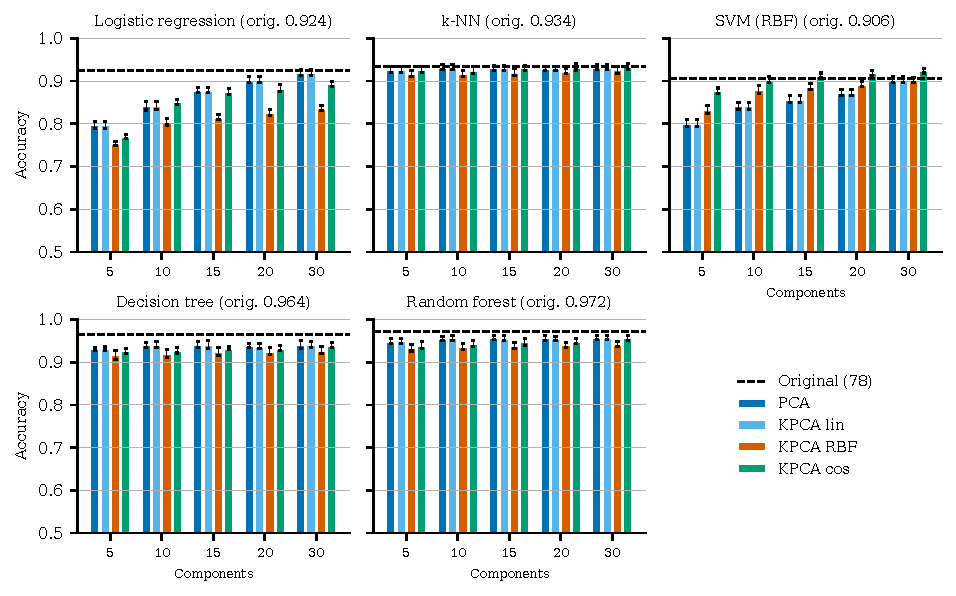
\includegraphics[width=0.55\textwidth]{figures/fig12_per_algorithm_accuracy.pdf}
\caption{Accuracy (mean $\pm$ std over 15 folds, standard class weights) of each classifier for PCA and KPCA at 5--30 components. Dashed line: original 78 features. The vertical axis starts at 0.5.}\label{fig:peralgo}
\end{figure}

\subsection{Selection optimism: nested cross-validation}\label{sec:results-nested}
Selecting the best of 189 configurations on the scoring folds is optimistic, so selection was repeated inside a nested cross-validation (Section~\ref{sec:method}). The configuration chosen on inner folds reached macro-F1 $0.900\pm0.022$ (accuracy 0.972, MCC 0.947) on the outer folds against 0.901 for the same-CV maximum: an optimism of about 0.0006. The inner folds chose an original-feature configuration in all 15 outer folds (RF 11 times, DT 4). Original features were clearly better than the inner-selected best reduced space for DT ($+0.093$) and RF ($+0.062$), similar for $k$-NN ($+0.002$). For logistic regression the macro-F1 difference was 0.004, smaller than the fold standard deviation of 0.022; its unadjusted Wilcoxon $p$ was 0.010, and because outer folds share training data it is exploratory. For the SVM the reduced space was better by 0.060 (cosine KPCA-30 was chosen in all 15 folds). The $p$-values are unadjusted.



\subsection{Effect of hyper-parameter tuning}
Table~\ref{tab:tuning} reports the nested search (five outer folds). Tuning barely changed the random forest (original 0.901 default, 0.899 tuned; best reduced 0.842 versus 0.839). For $k$-NN it added $+0.007$ on original features, and the gap to the best reduced space stayed within 0.003: 0.000 under defaults (cosine KPCA-30), $-0.002$ after tuning (PCA-30), and $+0.003$ for PCA-30 under defaults. All of these are far below the fold variation. The SVM changed most. Tuned macro-F1 rose from 0.668 to 0.791 on original features and from 0.745 to 0.812 with cosine KPCA-30, so the advantage of reduction shrank from 0.076 to 0.021. Five outer folds cannot establish a difference of 0.021, and the selected values sit on grid edges ($C=10$ for the SVM and $k=3$ for $k$-NN in all 20 selections). We therefore read the SVM advantage of KPCA as a property of the default RBF-SVM that largely disappears with tuning, not as a robust benefit of KPCA.

\begin{table}[!htbp]
\caption{Nested hyper-parameter search: mean macro-F1 over five outer folds. For each setting (default, tuned) the best reduced space among PCA-30, KPCA-cos-30 and KPCA-RBF-30 is chosen by that setting\textquoteright s own score; $\Delta$ = original $-$ reduced (negative: reduction better). K-cos-30 = KPCA, cosine kernel, 30 components. The last column gives the default-setting gap measured in the tuned-best reduced space.}\label{tab:tuning}
\centering\scriptsize
\resizebox{\textwidth}{!}{\begin{tabular}{lccrccrr}
\toprule
 & \multicolumn{3}{c}{Default settings} & \multicolumn{3}{c}{Tuned (nested search)} & \\
\cmidrule(lr){2-4}\cmidrule(lr){5-7}
Clf & Orig. & Best reduced & $\Delta$ & Orig.  & Best reduced  & $\Delta$  & $\Delta$ def., tuned-best space \\
\midrule
KNN & 0.801 & 0.801 (K-cos-30) & +0.000 & 0.808 & 0.810 (PCA-30) & -0.002 & +0.003 \\
SVM & 0.668 & 0.745 (K-cos-30) & -0.076 & 0.791 & 0.812 (K-cos-30) & -0.021 & -0.076 \\
RF & 0.901 & 0.842 (PCA-30) & +0.059 & 0.899 & 0.839 (PCA-30) & +0.060 & +0.059 \\
\bottomrule
\end{tabular}
}
\end{table}

\subsection{Row-order robustness (proxy chronology)}
In the head/tail split 4{,}199 records train and 1{,}769 test (32 test records of unseen classes were dropped); only seven of the 15 classes occur in both parts. The random forest on original features scored 0.838 versus 0.948 for a random split of the same rows and classes (decision tree 0.846 versus 0.959). For DT, RF and LR the reduced spaces lost at least as much (RF: PCA-10 0.759, cosine KPCA-30 0.704), so original $>$ reduced was preserved; $k$-NN stayed a near tie (0.790 versus 0.806) and the SVM again favoured cosine KPCA-30 (0.616 versus 0.479). In blocked cross-validation (6--10 classes scored per fold) the random forest scored 0.851 versus 0.932 for random folds, with the original space again ahead for DT, RF and LR. Both checks assume that row order follows capture time and score only some classes, so they support the ranking but give no precise penalty.





\subsection{Kernel, component count and class weighting}
Linear KPCA reproduced PCA, as expected on centred data: results were identical for $k$-NN and SVM and within 0.001 (LR) or 0.007 (trees). For LR and SVM the number of components mattered more than the kernel (LR macro-F1 rose from 0.37 at 5 PCA components to 0.73 at 30, against 0.736 on original features). For the SVM cosine KPCA was best (mean macro-F1 0.657 versus 0.536 linear and 0.515 RBF; $\gamma$ untuned). Balanced class weights raised balanced accuracy for LR and SVM but lowered macro-F1 for LR (0.736 $\to$ 0.710) and RF (0.901 $\to$ 0.885), so the best model remained the unweighted random forest.

\subsection{Computational cost}
The serial benchmark (table in the repository; separate from the per-fold fit times of the main grid) used 4{,}800 training and 1{,}200 test records. KPCA fitting took 5.5--5.6\,s against 0.02\,s for PCA, more than 200 times as long. It raised decision-tree training from 0.07\,s with PCA to 5.3--5.6\,s and random-forest training from 0.84--0.90\,s to 6.3--6.6\,s, and made random-forest inference about five times slower. Peak traced memory of the whole pipeline was 363\,MB for KPCA against 9.8\,MB for PCA or no reduction, about 37 times. It grew roughly quadratically with $n$ (3.1\,MB at $n=400$ to 359.1\,MB at $n=4800$), consistent with an $n\times n$ float64 kernel matrix (184\,MB at $n=4800$). By arithmetic, not measurement, a dense float64 kernel matrix for all 2{,}830{,}743 source flows would need about 64\,TB, so exact KPCA on the full data needs approximation or sub-sampling (not tested).







\subsection{Comparison with the five best surveyed papers}
Fig.~\ref{fig:cmp} places our best accuracy, 97.22\,\% for the random forest on the original features, beside the five best papers of Table~\ref{tab:lit} (97.6\,\% to 99.996\,\%). Our figure is the lowest of the six, so this work does not outperform those studies on accuracy, and the bars are not a like-for-like ranking. Their datasets, splits and balancing differ from ours, and most report accuracy from an abstract without class-level metrics. Our sample deliberately over-represents attack classes (benign is 67.2\,\% of the sample against 83\,\% of the de-duplicated pool), removes exact duplicates, and is scored by repeated cross-validation, and our macro-F1 of 0.901 is a stricter measure than accuracy. Qin~\cite{qin} shows the same gap: 0.9989 accuracy but 0.7114 macro-F1. The purpose of our study is not to beat these systems but to test whether PCA or KPCA adds anything to a given classifier.

\begin{figure}[!htbp]\centering
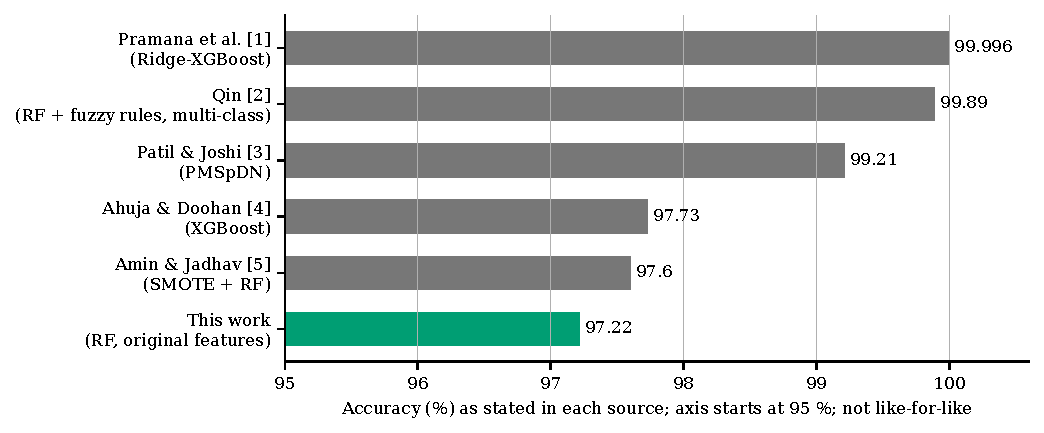
\includegraphics[width=0.8\textwidth]{figures/fig11_accuracy_comparison.pdf}
\caption{Accuracy of this work versus the five best surveyed IEEE Xplore papers (values as stated in each source). The horizontal axis starts at 95\,\%. Datasets, sampling designs and evaluation splits differ, so the bars are not a like-for-like ranking.}\label{fig:cmp}
\end{figure}

\subsection{Discussion}
\textbf{Best algorithm.} The random forest on the original 78 features achieved the highest accuracy (97.22\,\%) and the highest macro-F1 (0.901) of all 189 configurations. \textbf{Answers to the research questions.} RQ1 and RQ2: reducing to 5--30 components mostly did not help and usually lowered macro-F1, clearly for the decision tree and random forest and negligibly for logistic regression (30 components) and $k$-NN. The one gain, the RBF-SVM with cosine KPCA, largely disappeared under tuning (0.076 to 0.021). RQ3: the kernel mattered slightly more for $k$-NN, DT and RF, and the number of components for LR and SVM; default-$\gamma$ RBF was weakest for four of five classifiers. RQ4: at $n=4{,}800$, KPCA multiplied reducer fit time by more than 200 and traced memory by about 37, with no benefit for four of five classifiers. RQ5: orderings were stable across repeated folds, nested selection, tuning and the scorable row-order splits.

\textbf{Why accuracy misleads.} Benign flows are 67.2\,\% of the sample, so always answering ``benign'' scores 0.672. Yet the best model's 0.972 accuracy coexists with web-attack F1 of only 0.53 and 0.59; accuracy alone hides these weak classes.

\textbf{Possible explanations (untested).} We ran no experiment to separate these hypotheses. (i) Trees split on one feature at a time, so rotating the data into principal components may hide axis-aligned thresholds that trees exploit. (ii) PCA keeps the directions of largest variance, which need not separate rare classes such as the web attacks. (iii) A default RBF kernel with $\gamma=$ ``scale'' may suit the SVM poorly; the fall from 0.076 to 0.021 after tuning is consistent with this but does not prove it.

\subsection{Threats to Validity and Limitations}
The conclusions depend on the following limitations.

\textbf{1. Sample, not full data.} All results come from \emph{one} stratified sample of 6{,}000 records out of 2.5\,M de-duplicated flows (0.24\,\%) and the pipeline was run on a single sampling seed, not repeated over several samples, because exact KPCA is quadratic in memory. The sample has a floor of 100 records per class and is \emph{not} prevalence-preserving: attack classes are over-represented, so accuracy, macro-F1 and class priors do not describe deployment-time prevalence. Heartbleed (11 records), SQL injection (21) and infiltration (36) are complete but tiny, so their per-class estimates are very uncertain, and another sample could change rankings that differ by a few points.

\textbf{2. Leakage status.} Sampling was performed on the raw, un-imputed data, and imputation, scaling and reduction are fitted inside each training fold. Remaining possible leakage channels were \emph{not} eliminated: records from the same attack session or burst can still fall into both training and test folds in the random 5-fold design, and near-duplicate (not exact-duplicate) flows are not removed.

\textbf{3. Limited external validity.} All data come from one dataset captured in one testbed over one week. The row-order checks score only seven classes (head/tail split) or six to ten classes per fold (blocked) and there is no cross-dataset evaluation.

\textbf{4. Selection and inference.} The headline configuration (RF, original features) was the best of 189 on the same cross-validation that produced its score. The nested analysis shows the optimism is about 0.0006 macro-F1 here, but the nested estimate itself is conditioned on the same sample. Repeated-CV significance tests violate independence; $p$-values are screening evidence, and unadjusted values are reported for the nested comparisons.

\textbf{5. Limited tuning.} Tuning covered only $k$-NN, SVM and random forest, four spaces and five outer folds, with small grids whose optimum lay on the edge for $k$-NN and SVM $C$. Logistic regression, the decision tree and the KPCA kernel parameters were not tuned, so conclusions about those concern default settings.

\textbf{6. Dataset quality and cost.} The original CIC-IDS2017 flows contain labelling and feature-construction artefacts and leakage problems that other studies discuss \cite{pramana,jiwueze}, which may distort scores (and may explain the web brute-force/XSS confusion); we did not use a corrected release. Timings and memory come from one 2-vCPU virtual machine, and memory is a traced lower bound.



We claim no new algorithm, state-of-the-art, real-time or production-ready performance, or generalisation beyond this sample. On this sample, original features were at least as good as PCA or KPCA for four of five classifiers. The one exception largely vanished with tuning. And accuracy hid a systematic failure on web attacks.

\section{Conclusion}
This paper asked whether PCA or KPCA improves intrusion detection over the 78 original CIC-IDS2017 features, using a class-stratified sample of 6{,}000 flows, five classical classifiers and repeated, nested and row-order validation. The highest accuracy was 97.22\,\% (macro-F1 $0.901\pm0.020$; $0.900\pm0.022$ with nested selection), and it came from the random forest on the original features, so reduction mostly did not help: it clearly hurt the decision tree and random forest and at best matched the original features for logistic regression and $k$-NN. Only the RBF-SVM gained, from cosine KPCA, and that gain shrank from 0.076 to 0.021 after tuning, while KPCA needed more than 200 times the reducer fit time and about 37 times the traced memory of PCA. Accuracy hid weak detection of web brute force and XSS (F1 0.53 and 0.59). These findings apply only to this one sample of CIC-IDS2017; future work should repeat the pipeline over several sampling seeds and larger samples, add cross-dataset evaluation and widen the tuning grids.

\section*{Data and Code Availability}
The raw CIC-IDS2017 MachineLearningCVE files are distributed by the dataset provider (the Canadian Institute for Cybersecurity) and are not redistributed here. The code, per-fold results, tables and figures \ifdefined\BLIND are kept in an anonymised repository whose link will be supplied after review.\else are available in the \texttt{research-ieee} branch of \url{https://github.com/Gowtham-212007/ACN-PROJECT-V2}.\fi


\section*{Acknowledgments and AI-assistance disclosure}
Generative AI was used in this work. Claude (Anthropic; Claude Code, model Claude Sonnet 5.5) helped (i) write and revise the Python pipeline (data preparation, validation, statistics, benchmarks, tables, figures and a claim checker); (ii) draft and edit the text of all sections, including the abstract, captions and limitations; and (iii) check bibliographic details and statements attributed to sources. ChatGPT (OpenAI) gave editorial suggestions and extra source checks. All reported numbers were produced by code run on the data described and re-checked by script. The authors reviewed the content and remain fully responsible for it. The authors received no specific funding for this work and declare no competing interests.

\bibliographystyle{unsrt}
{\let\small\footnotesize\bibliography{references}}
\end{document}
